% Requires \usepackage{tikz} and \usepackage{xcolor} in the preamble.
% Full-page-bleed Decision Stack: pyramids clip at the physical page edges.

\makeatletter
\definecolor{diag@gold}{RGB}{184,146,42}
\definecolor{diag@goldlt}{RGB}{212,168,67}
\definecolor{diag@dark}{RGB}{37,36,34}
\definecolor{diag@medium}{RGB}{64,61,57}
\definecolor{diag@light}{RGB}{204,197,185}
\definecolor{diag@cream}{RGB}{255,252,242}
\definecolor{diag@muted}{RGB}{90,80,64}
\makeatother

\vspace{0.5em}
\noindent
\makebox[\textwidth][l]{%
\hspace*{-\dimexpr\oddsidemargin+1in\relax}%
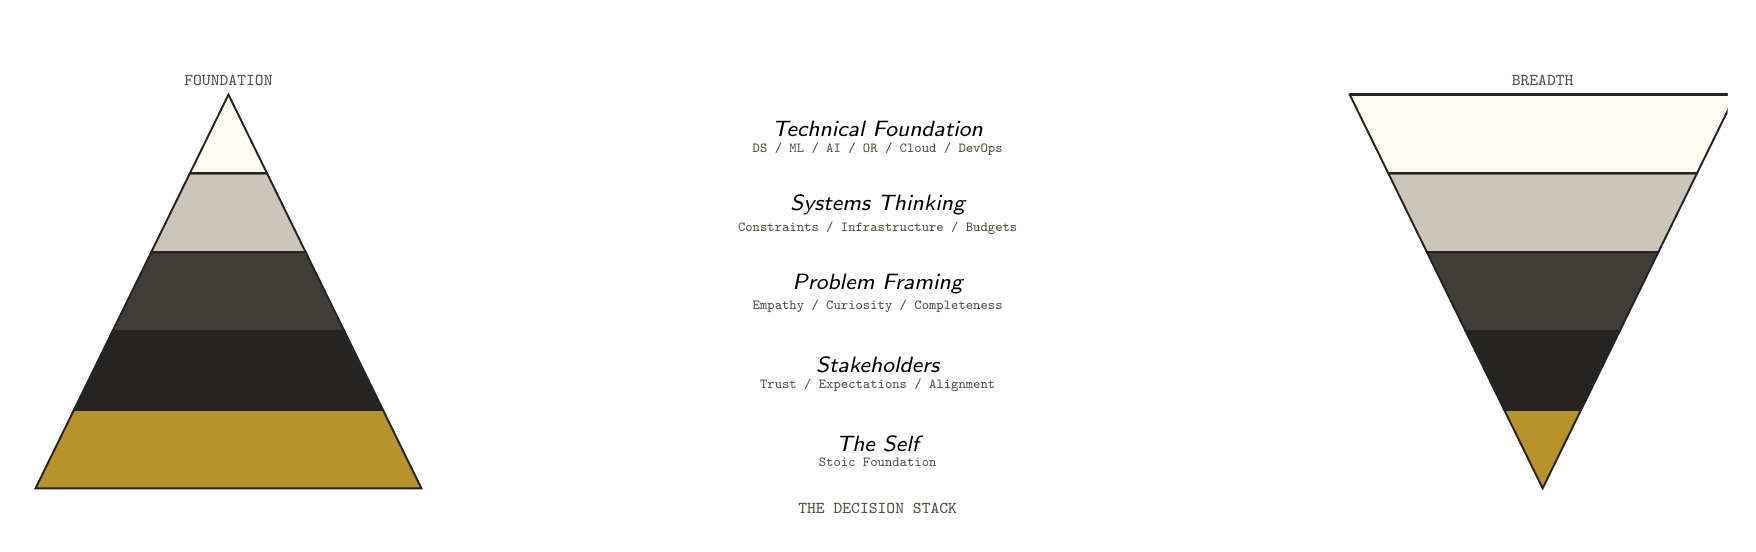
\begin{tikzpicture}[x=1cm, y=1cm, font=\sffamily]
  \pgfmathsetmacro{\W}{\paperwidth/1cm}
  \def\H{1.0}
  \pgfmathsetmacro{\Htot}{5*\H}
  % Foundation sits slightly closer to the labels than Breadth
  \pgfmathsetmacro{\hw}{2.45}
  \pgfmathsetmacro{\cxL}{2.55}
  \pgfmathsetmacro{\cxR}{\W-2.35}

  % Bounding box = clip window, so off-page vertices do not widen the picture
  \path[use as bounding box] (0,-0.45) rectangle (\W, 5.85);
  \clip (0,-0.45) rectangle (\W, 5.85);

  % ---- LEFT PYRAMID (upright; outer base bleeds off the left edge) ----
  \foreach \i/\lc in {1/diag@gold, 2/diag@dark, 3/diag@medium, 4/diag@light, 5/diag@cream} {
    \pgfmathsetmacro{\ybot}{(\i-1)*\H}
    \pgfmathsetmacro{\ytop}{\i*\H}
    \pgfmathsetmacro{\hwbot}{\hw*(1-\ybot/\Htot)}
    \pgfmathsetmacro{\hwtop}{\hw*(1-\ytop/\Htot)}
    \filldraw[fill=\lc, draw=diag@dark, line width=0.7pt, line join=miter]
      ({\cxL-\hwbot},\ybot) -- ({\cxL+\hwbot},\ybot) --
      ({\cxL+\hwtop},\ytop) -- ({\cxL-\hwtop},\ytop) -- cycle;
  }

  % ---- RIGHT PYRAMID (inverted; outer top bleeds off the right edge) ----
  \foreach \i/\lc in {1/diag@gold, 2/diag@dark, 3/diag@medium, 4/diag@light, 5/diag@cream} {
    \pgfmathsetmacro{\ybot}{(\i-1)*\H}
    \pgfmathsetmacro{\ytop}{\i*\H}
    \pgfmathsetmacro{\hwbot}{\hw*(\ybot/\Htot)}
    \pgfmathsetmacro{\hwtop}{\hw*(\ytop/\Htot)}
    \filldraw[fill=\lc, draw=diag@dark, line width=0.7pt, line join=miter]
      ({\cxR-\hwbot},\ybot) -- ({\cxR+\hwbot},\ybot) --
      ({\cxR+\hwtop},\ytop) -- ({\cxR-\hwtop},\ytop) -- cycle;
  }

  % Horizontal seams on top of each layer so cream/light read on white paper
  \foreach \i in {1,...,5} {
    \pgfmathsetmacro{\ytop}{\i*\H}
    \pgfmathsetmacro{\hwL}{\hw*(1-\ytop/\Htot)}
    \pgfmathsetmacro{\hwR}{\hw*(\ytop/\Htot)}
    \draw[diag@dark, line width=0.8pt]
      ({\cxL-\hwL},\ytop) -- ({\cxL+\hwL},\ytop);
    \draw[diag@dark, line width=0.8pt]
      ({\cxR-\hwR},\ytop) -- ({\cxR+\hwR},\ytop);
  }

  % Labels sit above each pyramid's center, which stays on the page
  \node[above, font=\fontsize{6}{7}\selectfont\ttfamily, text=diag@muted, inner sep=3pt]
    at (\cxL,\Htot) {FOUNDATION};
  \node[above, font=\fontsize{6}{7}\selectfont\ttfamily, text=diag@muted, inner sep=3pt]
    at (\cxR,\Htot) {BREADTH};

  % ---- CENTER TEXT COLUMN ----
  % Title sits just above the band midline, subtitle just below, so the pair
  % is tight and optically centered (a single \\ node sits too high).
  \foreach \ymid/\ttl/\sub in {
      4.43/{Technical Foundation}/{DS / ML / AI / OR / Cloud / DevOps},
      3.43/{Systems Thinking}/{Constraints / Infrastructure / Budgets},
      2.43/{Problem Framing}/{Empathy / Curiosity / Completeness},
      1.43/{Stakeholders}/{Trust / Expectations / Alignment},
      0.43/{The Self}/{Stoic Foundation}%
    } {
    \node[anchor=south, inner sep=1.2pt, outer sep=0pt, align=center]
      at ({\W/2}, \ymid)
      {\fontsize{8.5}{9}\selectfont\itshape \ttl};
    \node[anchor=north, inner sep=1.2pt, outer sep=0pt, align=center]
      at ({\W/2}, \ymid)
      {\fontsize{5.5}{6}\selectfont\ttfamily\color{diag@muted} \sub};
  }

  \node[anchor=north, font=\fontsize{6}{7}\selectfont\ttfamily, text=diag@muted,
        inner sep=2pt]
    at ({\W/2}, -0.12) {THE DECISION STACK};
\end{tikzpicture}%
}
